\documentclass[12pt,a4paper]{report}
\usepackage[ascii]{inputenc}
\usepackage{amsmath}
\usepackage{amsfonts}
\usepackage{indentfirst}
\usepackage{amssymb}
\usepackage{graphicx}
\usepackage{csquotes} 
\author{Iskhakov Anas, Thologelo Mphahlele, AbdurRahman El Gammal}

\begin{document}
\title{ Essential Skills Lab-4 }
	\author{Thologelo, Anas, AbdurRahman}
	\date{September 20, 2017}
\maketitle
	\tableofcontents
	\chapter{Thologelo's Part WIKI}
	\section{What is a Wiki?}
	The name "Wiki" was chosen by Ward Cunningham - the creator of the first Wiki. It is a shortened form of "wiki- wiki", the Hawaiian word for quick. A wiki is a web site that is generally editable by anyone with a computer, a web browser, and an internet connection. Wikis use a quick and easy syntax to allow users to apply formatting to text and create links between pages. This simple formatting syntax means that authors no longer need to learn the complexities of HTML to create content on the web. The main strength of a wiki is that it gives people the ability to work collaboratively on the same document. The only software you need is an Internet browser. Consequently, wikis are used for a variety of purposes. If you make a mistake, it's easy to revert back to an earlier version of the document. 

	\begin{figure}[h]
		\centering
		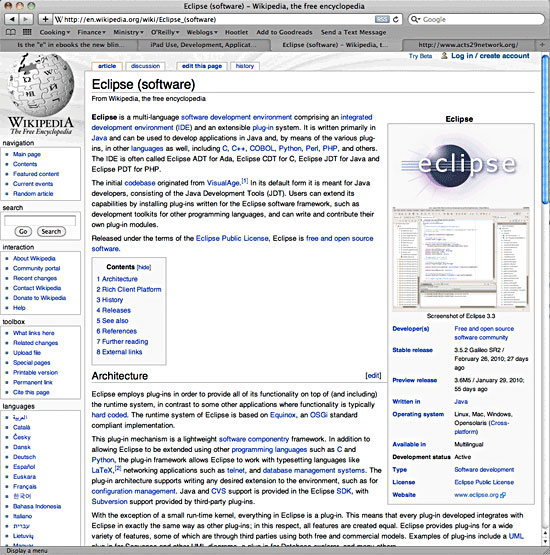
\includegraphics[width=10cm]{wikiexample.jpg}
		\caption{Example of WIKI page.}
	\end{figure}

	The largest and most talked about Wiki on the Internet is Wikipedia. Wikipedia is, for the most part, editable by anyone in the world with a compute and aninternet connection and, at the time of this writing, contained over 1,500,000 pages. One and a half million pages in English. There are also more than 250,000 articles in another languages While Wikipedia's mission is to create an encyclopedic resource of knowledge, wikis can be used for a variety of purposes and are quickly becoming the defacto technology for collaborative group work online. They can be great social tools for classrooms, teams, community groups, or can even be configured to provide easily updatable web sites for organizations. \cite{wiki}


\newpage
	\subsection{Advantages}
\begin{itemize}
	\item Anyone can edit,
	\item easy to use and learn,
	\item Wikis are instantaneous so there is no need to wait for a publisher to create a new edition or update information,
	\item people located in different parts of the world can work on the same document.
\end{itemize}	
	\subsection{Disadvantages}
	Advantages in one context, may be disadvantages in another.
\begin{itemize}
	\item Anyone can edit so this may be too open for some applications, for example
	confidential documentation. However it is possible to regulate user access,
	\item open to SPAM and Vandalism if not managed properly. There are easy ways to restore
	a page however, and on WikiEducator you must be logged in to edit pages so this
	reduces vandalism by automated spam bots,
	\item requires Internet connectivity to collaborate, but technologies to produce print versions of articles are improving,
	\item the flexibility of a wiki's structure can mean that information becomes disorganised.
\end{itemize}	

	\section{Wiki Community}
	As a wiki grows, the community plans and administers the structure collaboratively
	The values of our WikiEducator community 
	It is important to recognise and respect the core values of the different wiki communities.

	\itshape	The WikiEducator \normalfont 	community believes in the following values:
\begin{itemize}
	\item	The social inclusion and participation of all people in our networked society (Access to 	ICTs is a fundamental right of knowledge citizens - not an excuse for using old 	technologies).
	\item	The freedoms of all educators to teach with the technologies and contents of their choice, hence our commitment to Free/ Libre and Open Source technology tools and free content.
	\item	That educational content is unique - and by working together we can improve the technologies we use as well as the reusability of digital learning resources.
	\item	In a forward- looking disposition working together to find appropriate and sustainable 	solutions for e- learning futures. 	WikiEducators strive to be friendly and neighbourly. 
\end{itemize}		
	Our mantra is: 
\begin{displayquote}
	\textit{
		"Just try it! Our community will support you" 
	}
\end{displayquote}
	
	\section{Conclusion}
	Wikis can be powerful tools to facilitate collaborative work and the development of online communities. The ability for distributed individuals to contribute to the same document or project with just a web browser and a network connection has resulted in some amazing achievements of peer- produced content over recent years. The most notable example is 	Wikipedia but we are still in the early days of this technology and great things may come from a wide adoption of wiki technology from communities and groups interested in creating open resources. We hope that WikiEducator continues to grow as a place to facilitate and support the development of Open Educational Resources (OERs) and a place for communities of interested practitioners.


\chapter{Anas's Part Web Services}
	
\section{Web Services Explained}
	A web service is a service offered by an electronic device to another electronic device, communicating with each other via the World Wide Web. In a Web service, Web technology such as HTTP, originally designed for human-to-machine communication, is utilized for machine-to-machine communication, more specifically for transferring machine readable file formats such as XML and JSON. In practice, the web service typically provides an object-oriented web-based interface to a database server, utilized for example by another web server, or by a mobile application, that provides a user interface to the end user. Another common application offered to the end user may be a mashup, where a web server consumes several web services at different machines, and compiles the content into one user interface.
	Three specifications for Web Services are illustrated in this section: SOAP, REST, and JSON.\cite{WEB}
	\section{SOAP}
	All the messages shown in the above figure are sent using SOAP. SOAP essentially provides the envelope for sending the Web Services messages. SOAP generally uses HTTP, but other means of connection may be used. HTTP is the familiar connection we all use for the Internet. In fact, it is the pervasiveness of HTTP connections that will help drive the adoption of Web Services. More on SOAP and Messaging.
	SOAP was originally part of the specification that included the Web Services Description Language (WSDL) and Universal Description, Discovery, and Integration (UDDI). It is used now without WSDL and UDDI. Instead of the discovery process described in the History of the Web Services Specification section below, SOAP messages are hard-coded or genereated without the use of a repository. The interaction is illustrated in the figure below. 
	
		\begin{figure}[h]
			\centering
			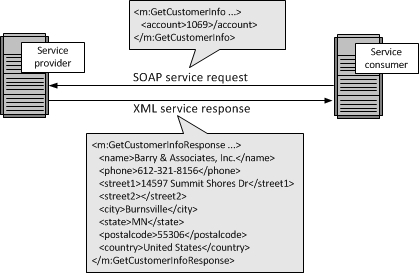
\includegraphics[width=10cm]{SOAP.jpg}
			\caption{Example of SOAP.}
		\end{figure}
\newpage	
	\section{REST}
\itshape	Representation State Transfer \normalfont  (REST) appeals to developers because it has a simpler style that makes it easier to use than SOAP. It also less verbose so that less volume is sent when communicating. The interaction is illustrated in the figure below. 
	
	\begin{figure}[h]
		\centering
		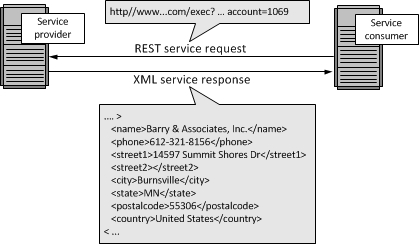
\includegraphics[width=10cm]{REST.jpg}
		\caption{Example of REST.}
	\end{figure}
	
	\section{JSON}
	While both SOAP and REST use XML for interchange,\itshape JavaScript Object Notation \normalfont (JSON) uses a subset of JavaScript. This is illustrated in the figure below. More on JSON.
	The most important advantage of services is that any system can work with them, be it a site, flash, program, etc., since the methods of parsing XML and executing HTTP requests are present almost 
	everywhere.
	
		\begin{figure}[h]
			\centering
			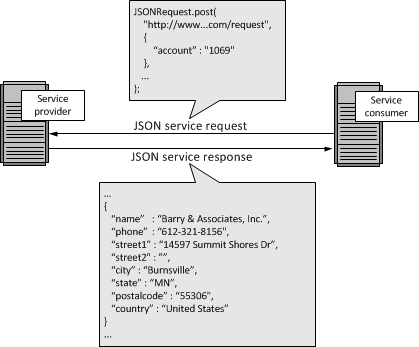
\includegraphics[width=10cm]{JSON.jpg}
			\caption{Example of JSON.}
		\end{figure}
\newpage	
	\section{Conclusion}
	The architecture of REST allows you to seriously simplify this task. Of course, in reality, the fact that described is not enough, because you can not give anyone the opportunity to change information, that is, you still need authorization and authentication. But this is quite simply solved by using different types of sessions or simply HTTP Authentication.
	
	
	
	
	\chapter{Abdur's Part LDAP}
	
	\section{History}

	LDAP was initially created by Tim Howes of the University of Michigan, Steve Kille of Isode Limited and Wengyik Yeong of Performance Systems International, circa 1993. It is based on the X.500 standard, but is simple and easily adapts to meet custom needs whose specifications are defined in the Requests for Comments (RFCs).\cite{LDAP}

	\section{What is it?}


	LDAP, \itshape Lightweight Directory Access Protocol\normalfont, is an Internet protocol that email and other programs use to look up information from a server.
	
	LDAP is mostly used by medium-to-large organizations. If you belong to one that has an LDAP server, you can use it to look up contact info and the like. Otherwise, if you were just wondering about this acronym, you probably don't need it. But feel free to read on to learn the story of this bit of Internet plumbing.
	
	Every email program has a personal address book, but how do you look up an address for someone who's never sent you email? How can an organization keep one centralized up-to-date phone book that everybody has access to?
		\begin{figure}[h]
			\centering
			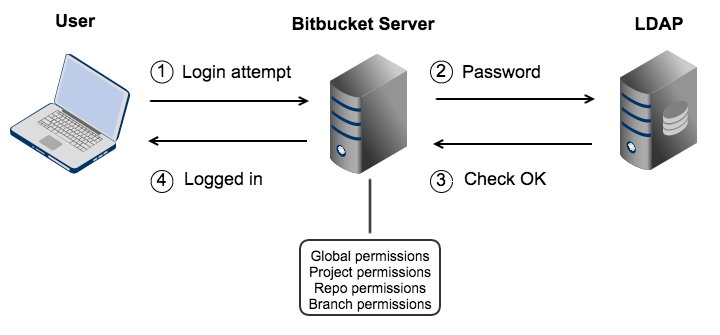
\includegraphics[width=10cm]{LDAP.png}
			\caption{Example of LDAP.}
		\end{figure}
	Those questions led companies such as Microsoft, IBM, Lotus, and Netscape to support a standard called LDAP. "LDAP-aware" client programs can ask LDAP servers to look up entries in a wide variety of ways. LDAP servers index all the data in their entries, and "filters" may be used to select just the person or group you want, and return just the information you want. For example, here's an LDAP search translated into plain English: "Search for all people located in Chicago whose name contains "Fred" that have an email address. Please return their full name, email, title, and description."
	
	LDAP is not limited to contact information, or even information about people. LDAP is used to look up encryption certificates, pointers to printers and other services on a network, and provide "single sign-on" where one password for a user is shared between many services. LDAP is appropriate for any kind of directory-like information, where fast lookups and less-frequent updates are the norm.
	
	\section{How does it work?}
	As a protocol, LDAP does not define how programs work on either the client or server side. It defines the "language" used for client programs to talk to servers (and servers to servers, too). On the client side, a client may be an email program, a printer browser, or an address book. The server may speak only LDAP, or have other methods of sending and receiving data?LDAP may just be an add-on method.
	
	If you have an email program (as opposed to web-based email), it probably supports LDAP. Most LDAP clients can only read from a server. Search abilities of clients (as seen in email programs) vary widely. A few can write or update information, but LDAP does not include security or encryption, so updates usually require additional protection such as an encrypted SSL connection to the LDAP server.
	
	If you have OS X and access to an LDAP server, you can enter your LDAP account into System Preferences--Internet Accounts. At bottom of the right pane, click Add Other Account, then choose the LDAP account option. This lets Address Book look up info from your server.




	
	\begin{thebibliography}{0}
		\bibitem{wiki} Stas Litvinov
		\emph{SNE Presentation Wiki}. Innopolis, September, 2017.
		\bibitem{WEB} Stas Litvinov
		\emph{SNE Presentation Web Services}. Innopolis, September, 2017
		\bibitem{LDAP} Rasheed Hussain
		\emph{SNE Presentation LDAP}. Innopolis, September, 2017
		
	\end{thebibliography}
	
\end{document}